\chapter{Implementation}%Jens
Due to the agile nature of the prototype development the implementation stage begun while the design phase was still underway. This chapter describes what went into the implementation of the final prototype.

\section{Micro controllers}%Daniel
	Initially doing the implementation phase, research went into what kind of micro controller, if any, we would need to construct a working prototype. Initially we settled for an Arduino Mega 2560, but going into the production phase, we realized that an external sound source was needed. The beaglebone black with the bela shield suited this purpose, and was taken in during this process.
	\subsection{Arduino}%Daniel
		
		
	\subsection{Bela}%Jens
		
	
\section{Code}
	\subsection{Arduino}%Daniel
		\subsubsection{Libraries}%Daniel
	\subsection{PureData}%Jens
	\begin{figure}[H]
		\centering
		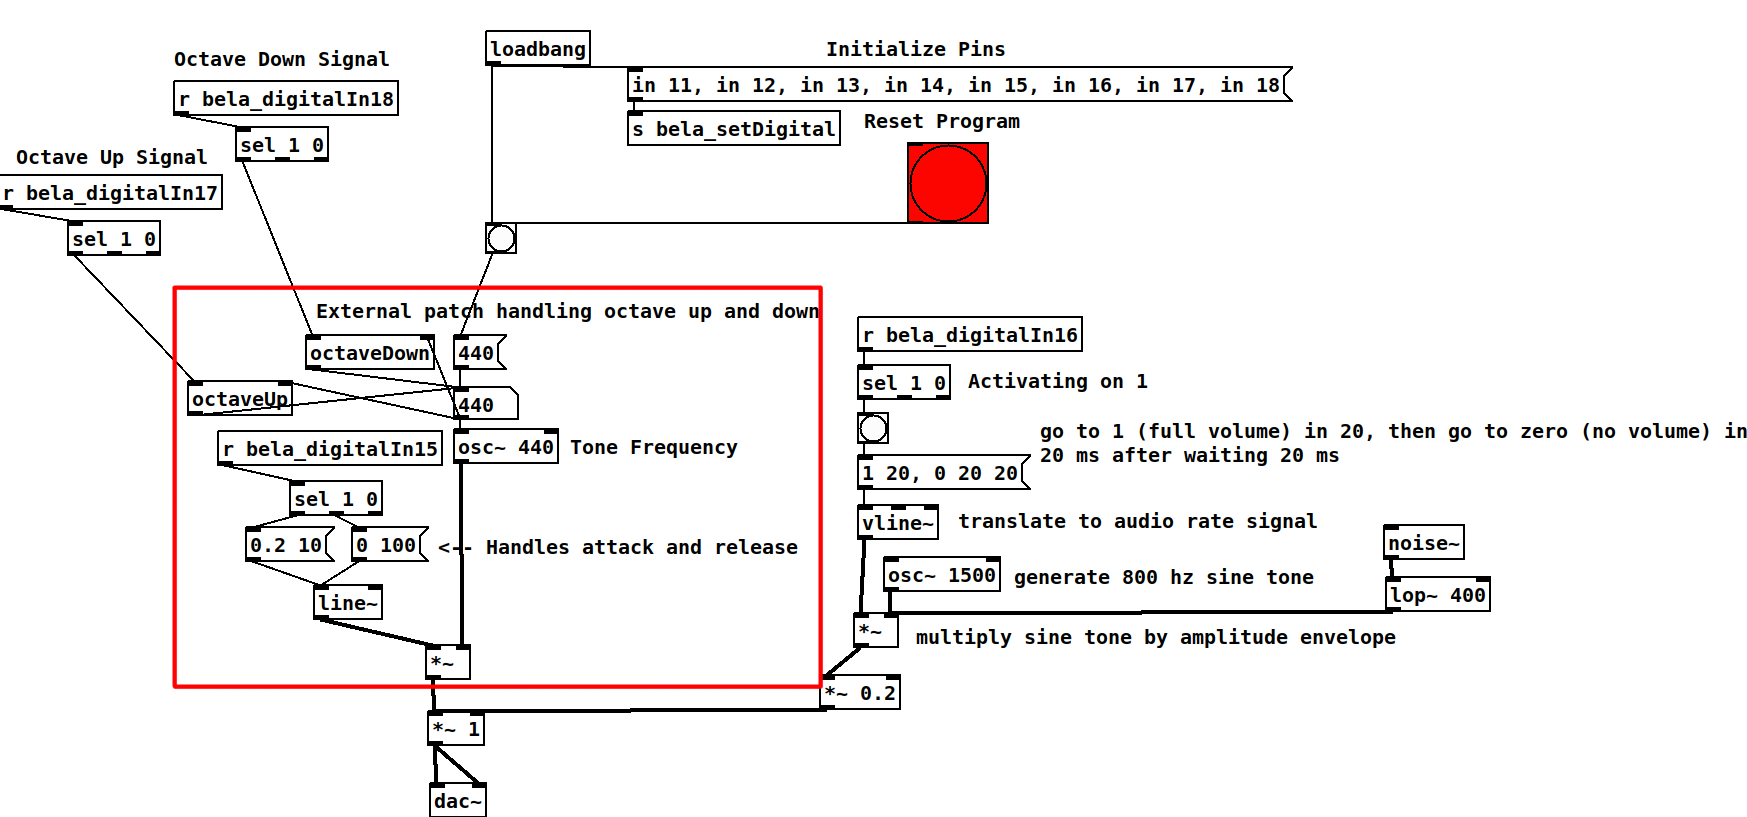
\includegraphics[width=1\linewidth]{figure/Implementation/pdPatch}
		\label{fig:pdPatch}
		\caption{Figure showing the main Pure Data patch for the prototype}
	\end{figure}	
	
\section{Circuit}


\section{The box}%Jens

	\subsection{CAD}
		
	\subsection{Assembly}

\section{The mat}%Daniel

\begin{listing}[H]
	\caption{Example 1}
	\label{listing:example1}
	\begin{minted}[frame=lines,framesep=2mm,baselinestretch=1.1,fontsize=\footnotesize,linenos]{cpp}
extern "C" __declspec( dllexport ) int init(int w, int h);
	\end{minted}
\end{listing}